\documentclass[twocolumn,10pt]{article}
\usepackage[letterpaper,left=1.95cm,right=1.95cm,top=2.5cm,bottom=3.16cm]{geometry}
\usepackage{natbib}
\usepackage{hyperref}
\usepackage{enumitem}
\usepackage{balance}
\usepackage{booktabs}
\usepackage{graphicx}
\usepackage{amsmath}
\usepackage{amssymb}
\usepackage[utf8]{inputenc}
\usepackage{wasysym} % symbols
\usepackage{amssymb} % symbols
\usepackage{abstract}
\usepackage{parskip}
\usepackage{hyperref}
\usepackage{titlesec}
\usepackage{xcolor}
\usepackage{natbib}
\usepackage{float}
\usepackage{graphicx}
\usepackage{fancyhdr}
\usepackage{titling}
\usepackage{caption}
\usepackage[document]{ragged2e}
\usepackage[affil-sl]{authblk} 
\usepackage{mathptmx}  %Times new Roman

\setlength{\columnsep}{1cm}
\renewcommand{\refname}{BIBLIOGRAFÍA}
\renewcommand{\figurename}{Fig.}
\renewcommand{\tablename}{Tabla.}
\renewcommand{\abstractname}{RESUMEN}

% Keywords command
\providecommand{\keywordsSpan}[1]
{
  \small	
  \textbf{\textit{Palabras Clave:}} #1
}

\providecommand{\keywordsEng}[1]
{
  \small	
  \textbf{\textit{Keywords:}} #1
}


%%%%%%%% FORMATO DE LAS SECCIONES Y SUBSECCIONES %%%%%
\titleformat{\section} 
	{\normalfont\large\bfseries}{\makebox[30pt][l]{\thesection}}{0pt}{} 
\titleformat{\subsection} 
	{\normalfont\large\bfseries }{\makebox[30pt][l]{\thesubsection}}{0pt}{}
\renewcommand\thesection{\arabic{section}.}
\renewcommand\thesubsection{\thesection\arabic{subsection}}
%%%%%%%% FORMATO DE LAS SECCIONES Y SUBSECCIONES %%%%%


	
\makeatletter
\long\def\@makecaption#1#2{
\vskip\abovecaptionskip
\sbox\@tempboxa{#1. #2}
\ifdim \wd\@tempboxa >\hsize
#1. #2\par
\else
\global \@minipagefalse
\hb@xt@\hsize{\hfil\box\@tempboxa\hfil}
\fi
\vskip\belowcaptionskip}
\makeatother


\pagestyle{fancyplain}% <- pagestyle fancyplain

\fancyfoot[C]{}
\renewcommand\plainheadrulewidth{.4pt}% headrule on plain pages
%\fancyhf{}
\rhead{Semestre 4 Año 2026}
\lhead{Estadística Bayesiana}
\rfoot{\thepage}

\date{}
 

%%%%%%% ENCABEZADO %%%%%%%%%%%%%%%%%%%%

{\title{\fontsize{16}{16}\selectfont
\vspace*{-0.7cm}
\textbf{
Entrega 02: Diseno Metodológico y EDA - Proyecto CS:GO
} \\[0.2cm]
\fontsize{12}{12}\selectfont
\textbf{Prediciendo lo Impredecible: Un Acercamiento con Estadistica Bayesiana en CS:GO}\\[0.2cm]}
}

\author[1,*]{\fontsize{10pt}{10pt}\selectfont \textbf{Julian Duarte}}
\author[2]{\textbf{Julian Jimenez}}
\author[3]{\textbf{Tomas Rincon}}

\affil[1]{\fontsize{8pt}{8pt}\selectfont Pregrado Ciencia de Datos Universidad Externado, Bogotá - Colombia}
\affil[2]{Pregrado Ciencia de Datos Universidad Externado, Bogotá - Colombia}
\affil[3]{Pregrado Ciencia de Datos Universidad Externado, Bogotá - Colombia \vspace{0.2cm}} 
\affil[*]{julian.duarte2@est.uexternado.edu.co; julian.jimenez5@est.uexternado.edu.co; juan.rincon14@est.uexternado.edu.co}

\begin{document}

\twocolumn[
  \begin{@twocolumnfalse}
    \maketitle

    \begin{center}
        \textbf{RESUMEN}
    \end{center}
    Este documento nace de la necesidad de entender mejor la logica para ganar en el Counter-Strike profesional. Este juego es tan dinamico que incluso el equipo mas fuerte puede perder en cualquier ronda. Usando estadística bayesiana y probabilidades, exploramos miles de partidas para ver qué tan seguros podemos estar de una predicción. Nuestra meta es ir mas alla de los puntos finales y entender los datos que realmente impactan los resultados en el juego competitivo.
    \vspace{0.2cm}

    \keywordsSpan{Esports, Regresion Logistica, Bayesiano, CS:GO, EDA, Priors.}
    
    \vspace{0.6cm}
  \end{@twocolumnfalse}
]

\thispagestyle{fancyplain}

\section{PROFUNDIZACION DE LA ENTREGA 1}

\subsection{Problema y Pregunta de Investigacion Refinada}
Imagina la gran final de un torneo. Dos equipos muy buenos estan jugando, el marcador esta empatado y hay demasiada tension. En las pantallas vemos que un equipo tiene el mejor Rating del evento, pero el mapa que juegan es la debilidad de ellos y la fuerza de los rivales. Ahi nos surge una interrogante: ¿basta con tener un buen accuracy y talento individual para ganarle a las malas estadísticas que tienen en ese mapa? 

El problema de las predicciones de hoy en dia es que nos botan un \textit{accuracy} altísimo y nos hacen creer que ya sabemos quién va a ganar, olvidando que en el Counter-Strike todo cambia muy rapido. No es solo saber quién es mejor en papel, sino ver qué tan fragil es la parametrización cuando entra la presion del partido en vivo. Queremos pasar de un cálculo sencillo a medir en serio la incertidumbre. En esta mezcla de habilidad de jugadores y mapas nace nuestra pregunta:

\textbf{Pregunta de investigacion:} ¿Como influyen el Rating de los equipos y el mapa que juegan en el desenlace de la partida en CS:GO, y cómo logramos sacar la probabilidad de esto usando distribuciones posteriores para medir la incertidumbre?

\subsection{Revision de Literatura Fortalecida}
Al leer otras investigaciones de esports \citep{hltv2024}, vimos algo que casi todos ignoran: los modelos solo buscan tener el mayor \textit{accuracy} asumiendo que las partidas son algo obvio a predecir. Este vacio ignora que en el juego no siempre gana el favorito, y esa incertidumbre es un dato clave \citep{csgodataset2020}. No existe un buen proyecto que use variables e intervalos para revisar qué tan confiable es el modelo.

Nuestro trabajo llenará este vacio con un analisis usando enfoques bayesianos guiado por dos métricas:

\textbf{Brier Score:} Esta metrica revisa la calidad de nuestras predicciones y penaliza si el modelo esta muy seguro de algo que fue un error.

\textbf{Intervalos HDI (Highest Density Interval):} Usando la distribucion posterior, este intervalo HDI refleja exactamente en qué posibles valores cae nuestra probabilidad de exito, dandole al modelo un indicador de duda muy realista \citep{kruschke2014doing}.

\section{METODOLOGIA}

\subsection{Enfoque del Estudio}
El proyecto utiliza estadística bayesiana para pronosticar los encuentros. Fuimos por este lado porque nos facilita cruzar datos e historias previas usando \textit{priors} con los números jugados en tiempo real. Esto es importante ya que nos saca no solo el resultado final de quién gana, sino el error e incertidumbre con el que lo calcula \citep{gelman2013bayesian}.

\subsection{Datos}
Alimentamos nuestro estudio con el dataset de nivel profesional llamado \texttt{csgo\_games.csv}. Ahi están guardadas más de 3700 peleas oficiales verificadas por la comunidad. La tabla tiene estadisticas univariadas y bivariadas de cada equipo y como se movieron esos numeros en vivo.

\begin{table}[!ht]
\centering
\caption{Variables clave del Dataset.}
\label{tab:data_dictionary}
\begin{tabular}{lp{5.2cm}}
\toprule
\textbf{Categoría} & \textbf{Atributos (Variable Técnica)} \\
\midrule
\textbf{Generales} & Equipos (\textit{team\_1/team\_2}) y ganador (\textit{winner}). \\
\textbf{Fuerza} & Rango HLTV (\textit{t1\_world\_rank}) y victorias (\textit{t1\_h2h\_win\_perc}). \\
\textbf{Habilidad} & Calificación (\textit{rating}), Impacto (\textit{impact}) y Daños (\textit{dmr}). \\
\textbf{Acción} & Bajas (\textit{kpr}) y Muertes (\textit{dpr}) por ronda. \\
\textbf{Escenarios} & Bajas de entrada (\textit{opk\_rating}) y clutch. \\
\bottomrule
\end{tabular}
\end{table}

\subsection{Estrategia del Metodo}
Nosotros construimos la base haciendo estos pasos principales:
\begin{enumerate}
    \item \textbf{Limpieza de Datos:} Eliminamos filas raras (\textit{outliers}), nulos y juegos que se cayeron. Ajustamos promedios de los jugadores para obtener variables de equipo (como \textit{t1\_rating\_avg}).
    \item \textbf{Asignar Priors:} Antes de correr algo, metimos \textit{priors} fijados según la diferencia de ranking de los equipos (\textit{t1\_world\_rank}) para darle contexto histórico al cálculo.
    \item \textbf{Muestreo de Simulaciones (NUTS):} Para generar la distribución posterior usamos el algoritmo NUTS, que ayuda a explorar las variables y llegar rápido a los parámetros que más explican quién ganó el mapa.
\end{enumerate}

\subsection{Seleccion del Modelo}
Utilizamos la \textbf{Regresion Logistica Jerárquica Bayesiana} porque nos ayuda con varias cosas del proyecto:
\begin{itemize}
    \item \textbf{Binario:} Como los partidos solo tienen victoria (1) o derrota (0), la logistica es muy facil de encajar en el target (\textit{target\_win}).
    \item \textbf{Priors:} Las \textit{priors} equilibran los huecos estadisticos si un equipo es nuevo o jugó poco.
    \item \textbf{Jerárquica (\textit{Partial Pooling}):} Permite prestar fuerza estadística entre grupos de datos parecidos (por ejemplo, entre distintos mapas o equipos) para evitar el sobreajuste.
\end{itemize}

\subsection{Limitaciones del Proyecto}
Por mas que los modelos sean buenos, existen problemas con las bases del juego: factores emocionales que los datos no ven, cambios del meta por parches de Valve y cambios rapidos de jugadores (\textit{roster changes}).

\section{ANALISIS EXPLORATORIO DE DATOS (EDA)}

\subsection{Pregunta y Subpreguntas Analiticas}
\textbf{Pregunta principal:} ¿Cuales estadisticas técnicas pronostican mejor un triunfo sobre una derrota de los equipos?
\begin{itemize}
    \item \textbf{S1:} ¿Como fluctua y qué impacto nos da la ventaja del mapa jugado?
    \item \textbf{S2:} ¿Será mejor guiarnos parametrizando un modelo basado en el Diferencial del Rating (\textit{rating\_diff}) antes que en el Impacto (\textit{impact\_diff})?
\end{itemize}

\subsection{Analisis Univariado y Bivariado}
Iniciando la inspección cruda, graficamos los atributos mecanicos. El $KPR$ (\textit{t1\_kpr\_avg}) y el Diferencial de Rating (\textit{rating\_diff}) muestran campanas casi normales agrupadas en ceros (Figura \ref{fig:DistFig}).

\begin{figure}[!ht]
    \centering
    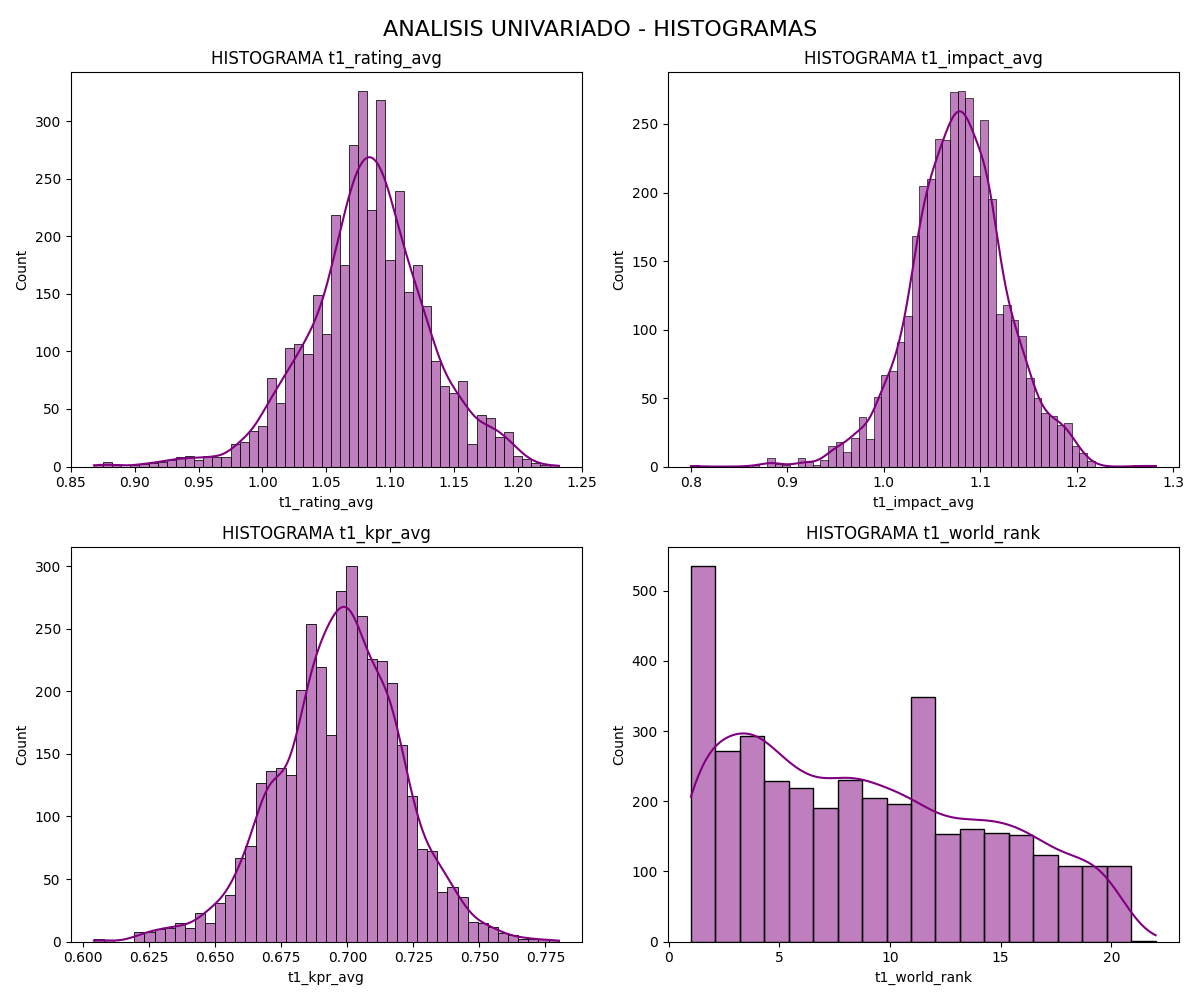
\includegraphics[width=\linewidth]{eda_univariado.png}
    \caption{Distribuciones Univariadas de variables tecnicas (Histogramas).}
    \label{fig:DistFig}
\end{figure}

Del mismo modo, analizamos el plano medioambiental (Figura \ref{fig:MapBiasFig}). Observamos que mapas como Nuke o Overpass muestran un sesgo marcado hacia el bando defensivo (\textit{ct\_winrate}), lo cual es una variable externa que el modelo debe parametrizar.

\begin{figure}[!ht]
    \centering
    
\includegraphics[width=\linewidth]{evidencia_mapa_bias.png}
    \caption{Sesgo de victoria del bando CT por mapa.}
    \label{fig:MapBiasFig}
\end{figure}

Al saltar a un analisis bivariado respecto a quien gana (\textit{target\_win}), revisamos las fluctuaciones con un analisis de cajas y violines cruzados (Figura \ref{fig:ViolinFig}) enfocados en el impacto (\textit{impact\_diff}). 

\begin{figure}[!ht]
    \centering
    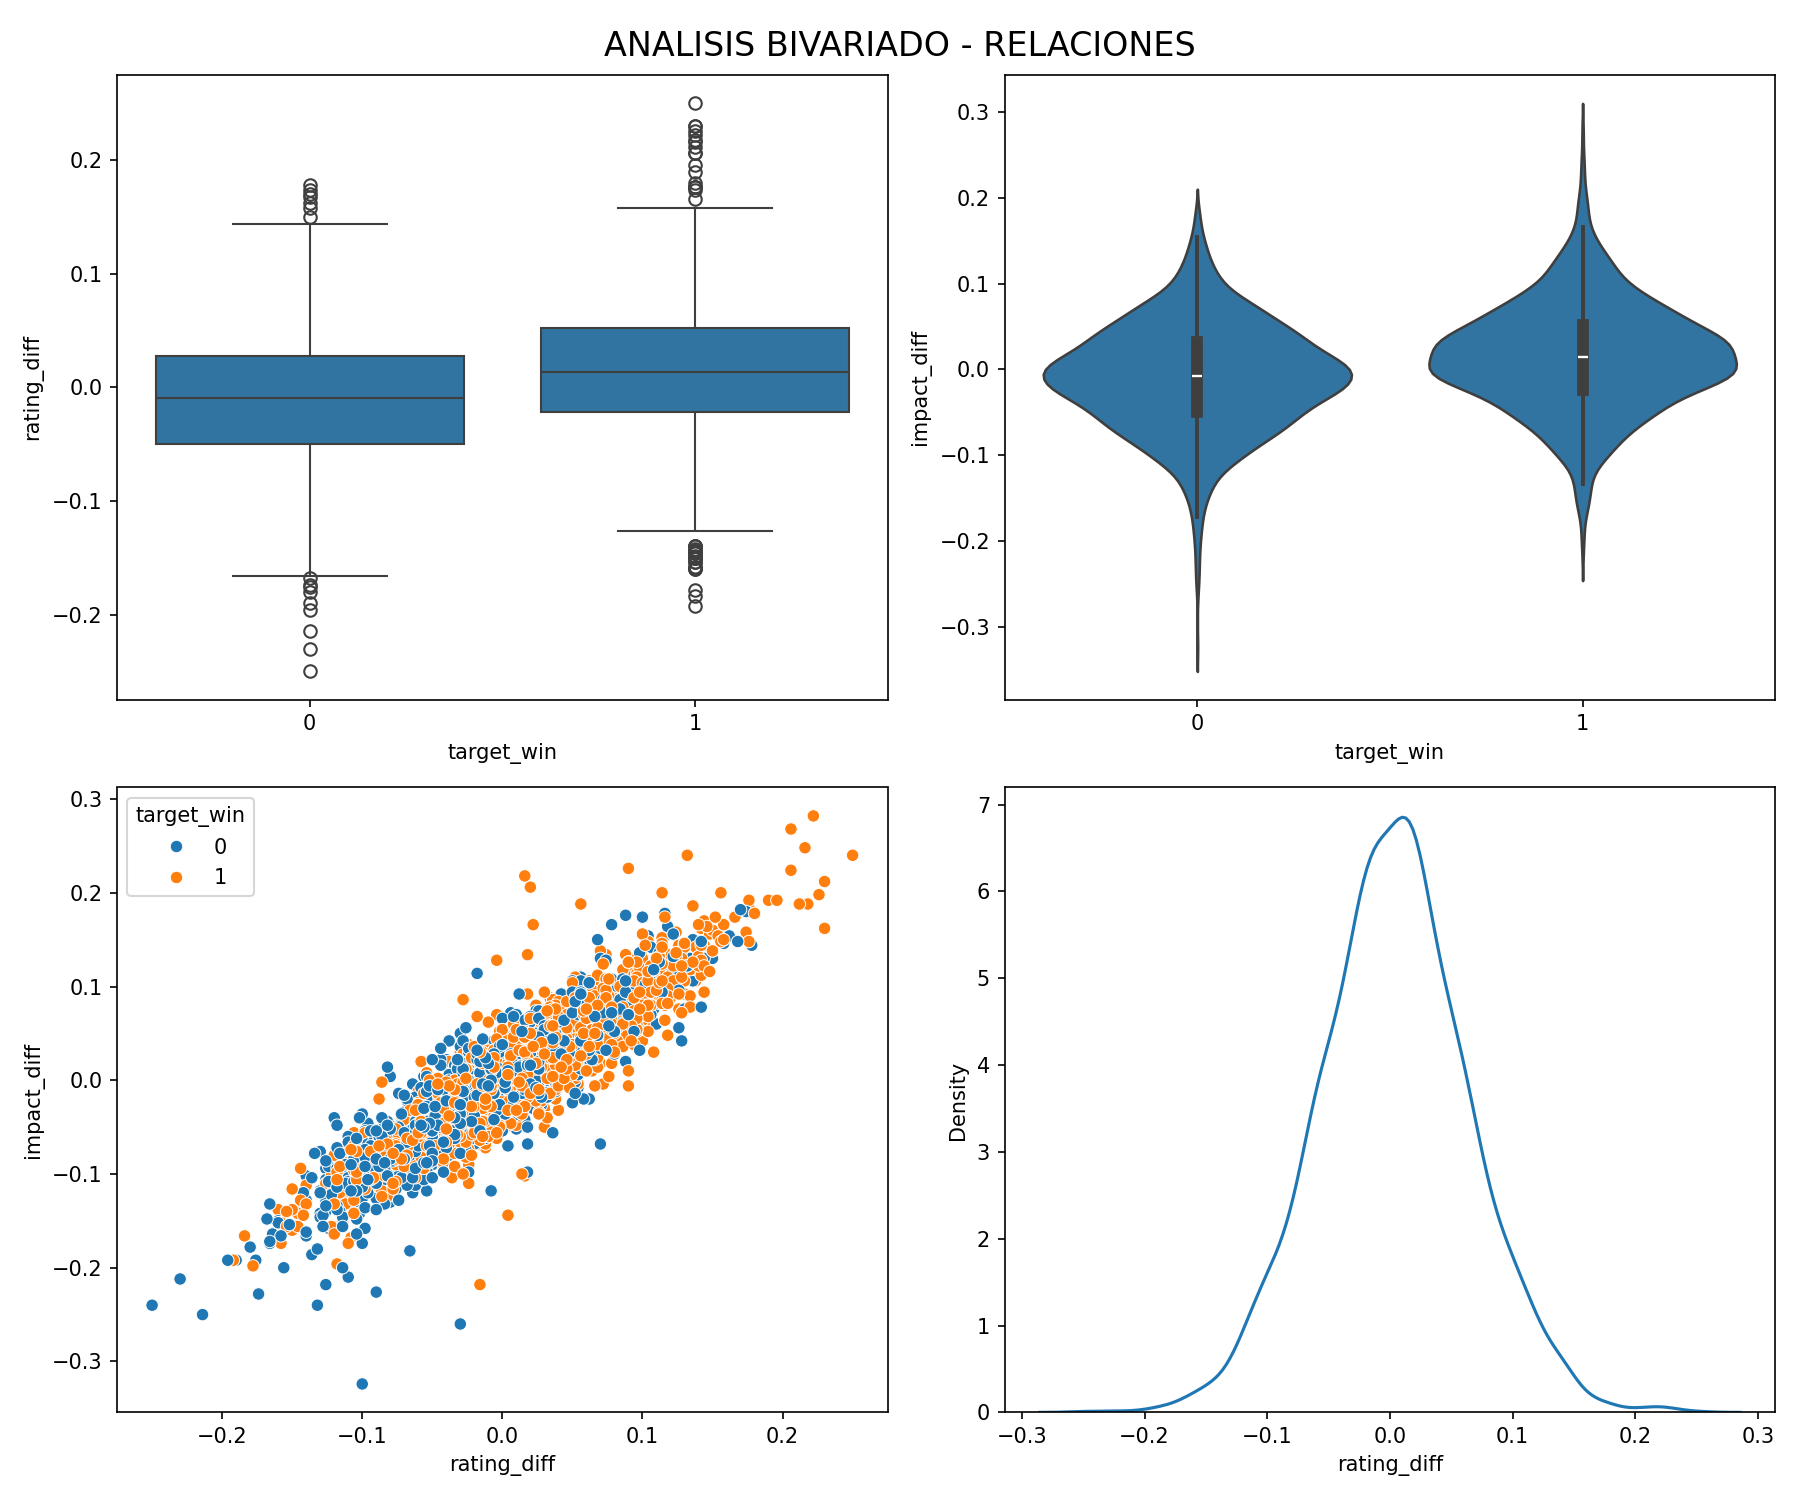
\includegraphics[width=\linewidth]{eda_bivariado_grid.png}
    \caption{Analisis Bivariado de Diferenciales (Rating, Impacto) vs Victoria.}
    \label{fig:ViolinFig}
\end{figure}

\subsection{Resultados e Interpretacion de EDA}

\begin{figure}[!ht]
    \centering
    
\includegraphics[width=\linewidth]{matriz_correlacion_completa.png}
    \caption{Matriz de Correlaciones de Pearson (Feature Selection).}
    \label{fig:CorrFig}
\end{figure}

Al calcular la matriz de correlación masiva con todos los parametros (Figura \ref{fig:CorrFig}), encontramos hallazgos tajantes. Variables que parecian utiles como el "Historial de victorias caras a cara" (\textit{t1\_h2h\_win\_perc}) o el "Rango Mundial" (\textit{t1\_world\_rank}) ni siquiera logran un impacto alto frente a la victoria. Por otro lado, observamos que los picos del Rating (\textit{rating\_diff}) marcan la pauta absoluta, dictando victoria directa con un grado alto de correlacion.

\subsection{Implicaciones al Modelar y Parametrizar}
Despues de la exploracion, nuestra regresión logística jerárquica va a necesitar unas \textit{priors} con mas varianza a la hora de meterle el impacto (\textit{impact\_diff}), ya que trae mucha volatilidad de datos. Pero con el Rating (\textit{rating\_diff}), que es un dato más constante, si vamos a poder trabajar con límites en modelos posteriores.

\bibliographystyle{apalike}
\bibliography{bibliografia}

\end{document}
